\documentclass[12pt]{iopart}
% Requires iopart.cls (IOP Publishing; NOT on CTAN). Compile on Overleaf
% (template "iopart") or with IOP's downloadable author template, which
% ship the class; iopart-num.bst is already in TeX Live. Prepared but NOT
% compiled locally (iopart.cls unavailable here). Body == condensed
% manuscript.tex.

\usepackage[T1]{fontenc}
\usepackage[utf8]{inputenc}
\usepackage{graphicx}
\usepackage{amsmath,amssymb}
\usepackage{bm}
\usepackage{siunitx}
\usepackage{booktabs}
\usepackage[numbers,sort&compress]{natbib}
\usepackage{xcolor}
\usepackage{hyperref}
\usepackage{xr-hyper}
\externaldocument{supplement}
\hypersetup{colorlinks=true, linkcolor=blue!50!black, citecolor=blue!50!black, urlcolor=blue!50!black}
\graphicspath{{figures/}}

\begin{document}

\title{A two-feedback Vicsek--Couzin flock: density-stratified heading correlations as the robust fingerprint of motility--noise coupling}

\author{Yaya Youssouf Yaya}
\address{D\'epartement de Math\'ematiques, \'Ecole Normale Sup\'erieure de N'Djam\'ena, BP~206, N'Djam\'ena, Tchad}
\address{Chercheur Associ\'e, LMA, U.F.R.~Sciences et Technologies, Universit\'e Assane Seck de Ziguinchor, BP~523, Diabir, Ziguinchor, S\'en\'egal}
\ead{yy.y@zig.univ.sn}

\begin{abstract}
The Vicsek model fixes the self-propulsion speed and the
angular-noise distribution as global constants. The
active-matter literature has relaxed each one separately: a
density-dependent speed drives motility-induced phase
separation, and heavy-tailed L\'evy reorientations reshape the
order--disorder transition. What happens when both adaptations
fire together has not been settled. We gate the speed and the
stability index of an $\alpha$-stable angular kick through one
shared sigmoid in the local neighbour count, so a crowded
particle is at once slow and Gaussian-like while an isolated
one is fast and Cauchy-like. A seven-size finite-size scan
against the original Vicsek model and three single-channel
ablations splits the problem in two. Heavy-tailed
reorientations on their own grow no size-dependent
susceptibility (their rare bursts wash out among the many
neighbours of a dense patch) whereas the motility channel
does, building a phase-separated dense phase whose finite-size
susceptibility grows in a motility-induced-phase-separation
manner rather than through a sharp critical divergence. On top
of that, the otherwise-silent noise-shape adaptation adds a
finite-size super-additive excess. The robust, scale-spanning
fingerprint of the coupling is microscopic: the
density-stratified heading correlation inside the dense phase,
its dynamic counterpart $C(\tau)$, and the per-particle turning
statistics all read out one mechanism. Inside the
motility-driven dense phase the noise-shape feedback rectifies
Cauchy bursts into Gaussian-like kicks, switching dense-phase
reorientation from heavy-tailed to Gaussian and the droplets to
ballistic transport. A decoupled-sigmoid sweep pins the
motility threshold as the sole control of the sign and
amplitude of the rectification, with the noise-shape threshold
staying passive.
\end{abstract}

\noindent\textit{Keywords}: active matter, Vicsek--Couzin model,
motility-induced phase separation, finite-size scaling, heavy-tailed
($\alpha$-stable) angular noise, flocking.

\maketitle

\section{Introduction}

The Vicsek model \citep{Vicsek1995} freezes two ingredients of
a self-propelled flock that biology keeps fluid: every particle
moves at the same speed, and every reorientation is drawn from
the same Gaussian. Neither assumption survives contact with
real collectives. Self-propulsion speed responds to local
crowding almost everywhere one looks: confluent epithelia
jam and arrest \citep{Bi2016}, swarming bacteria switch between
planktonic and biofilm regimes through quorum sensing, and
vehicular, pedestrian and animal traffic carry a pronounced
speed--density anti-correlation \citep{Greenshields, LWR}. The
turning statistics are no closer to Gaussian: heavy-tailed
L\'evy turns are documented in foragers, T-cells and swarming
bacteria \citep{Reynolds2018, Harris2012, Ariel2015}. A
biologically honest flocking model should let both inputs read
the local environment.

These two relaxations have so far been studied apart.
\citet{CatesTailleur2015} showed that a steep enough
density-dependent speed drives motility-induced phase
separation (MIPS) with no alignment at all, and
density-dependent motility is now a standard route to
clustering in active matter. Heavy-tailed angular noise has run
on a separate, L\'evy-driven track \citep{Eliazar2003,
Ariel2015}, where broadening the turning tails reshapes the
order--disorder transition of metric Vicsek dynamics. Switching
both adaptations on together, gated by the same local cue, has
to our knowledge not been resolved, and the question is not
academic. The two channels should interrogate each other
precisely inside the dense regions a flock builds: the noise
distribution sets how a particle escapes a local structure,
while the density-dependent speed builds that structure in the
first place. Coupling them could as easily cancel as reinforce,
and only a direct test can decide.

We couple the two adaptations in the most economical way
available: a single sigmoid in the local neighbour count gates
both the self-propulsion speed and the stability index of the
angular noise, so a crowded particle is at once slow and
Gaussian and an isolated one fast and Cauchy. Turning both
channels off recovers the original Vicsek dynamics. Two
single-channel ablations (a motility-only mode with adaptive
speed and fixed Cauchy noise, and a noise-shape-only mode with
fixed speed and noise interpolating from Cauchy to Gaussian)
isolate
each contribution against a shared heavy-tailed reference, and a
finite-size scan at fixed density ($\rho_0 = 2.22$, sizes up to
$L = 128$) places the four heavy-tailed modes and the Gaussian
Vicsek baseline on the same footing.

The two channels separate cleanly. Only the modes carrying the
density-dependent speed phase separate in space and grow a
finite-size susceptibility ($\chi_{\max} \sim L^{1.29}$ for
motility-only); heavy-tailed noise on its own leaves the
transition essentially Vicsek-like, its rare bursts washed out
by the many neighbours of a dense patch. Together the two
feedbacks do more than add. The noise-shape adaptation, silent
on its own, lends the motility-driven, MIPS-like scaling a
super-additive boost ($\chi_{\max} \sim L^{1.95}$ for the full
mode, an excess $\Delta_7 = +0.63$). The mechanism is local.
Inside the dense phase the shared sigmoid pushes the noise
toward Gaussian, so the Cauchy bursts that would otherwise
scramble local alignment are rectified into coherent kicks; the
effect sharpens the dense-quartile heading correlation (a gap
$\Delta g = +0.153$ against the motility-only ablation, null in
the dilute phase), fuses the dense mass into fewer and larger
clusters, and leaves the dilute phase alone. A decoupled-sigmoid
analysis (Sec.~\ref{sec:decoupled}) pins the control variable:
the motility threshold alone sets the sign and amplitude of the
rectification, the noise-shape threshold staying passive. The
density-triggered slowdown is the precondition: without the
dense phase it builds, the heavy-tailed rectification has
nothing to act on and erodes coherence instead of creating it.

Section~\ref{sec:model} defines the two-feedback model, its
ablations and the numerical protocol. Section~\ref{sec:results}
reports the global diagnostics (finite-size susceptibility,
density separation, number fluctuations), the parametric
analyses (behavioural plane, order-parameter distribution,
hysteresis) and the local diagnostics (density-stratified
heading correlations, cluster statistics, single-particle
dynamics and the decoupled-sigmoid dissection) that localise the
rectification to the dense phase. Section~\ref{sec:disc}
discusses the mechanism, its place in the literature and its
limits, and the appendix (Sec.~\ref{sec:hydro}) sketches a
hydrodynamic account of the dense-phase rectification.

\section{Model and methods}
\label{sec:model}

\subsection{Dynamics}

$N$ point particles live in a square box of side $L$ with
periodic boundaries; particle $i$ carries a position $\mathbf
x_i \in [0, L)^2$ and a heading $\theta_i \in (-\pi, \pi]$,
advanced synchronously through
\begin{equation}
\theta_i(t+1) = \theta_i^\star(t+1) + \xi_i(t),
\qquad
\mathbf x_i(t+1) = \mathbf x_i(t) + v_i(t+1)\,\vec e_i(t+1)
   \pmod L,
\label{eq:update}
\end{equation}
with $\vec e_i = (\cos\theta_i, \sin\theta_i)$. The desired
heading $\theta_i^\star$ follows the Couzin priority rule
\citep{Couzin2002} with the repulsion set $\mathcal R_i =
\{j \neq i : |\mathbf r_{ij}| < R_r\}$,
$\mathbf r_{ij} = \mathbf x_j - \mathbf x_i$, and the
alignment set $\mathcal A_i = \{j \neq i : R_r \le
|\mathbf r_{ij}| < R_a\}$, both sensed omnidirectionally.
There is no attraction zone: spatial cohesion in this model
comes entirely from the density-dependent motility (the MIPS
route), not from a Couzin cohesion term, and ``Couzin'' here
labels only the zonal repulsion-over-alignment priority rule.
Repulsion takes priority over alignment, alignment over
inertia:
\begin{equation}
\theta_i^\star(t+1) =
\begin{cases}
\arg\!\left(-\sum_{j \in \mathcal R_i}
   \mathbf r_{ij} / |\mathbf r_{ij}|\right),
   & \mathcal R_i \neq \emptyset, \\[4pt]
\arg\!\left(\sum_{j \in \mathcal A_i} e^{i\theta_j(t)}\right),
   & \mathcal R_i = \emptyset
   \text{ and } \mathcal A_i \neq \emptyset, \\[4pt]
\theta_i(t),
   & \mathcal R_i = \mathcal A_i = \emptyset.
\end{cases}
\label{eq:theta_star}
\end{equation}
Interactions run in $O(N)$ on a cell-list partition.

The angular kick $\xi_i$ is a symmetric $\alpha$-stable variate
with a particle-dependent stability index,
\begin{equation}
\xi_i(t) \sim S_{\alpha_i(t)}\bigl(c = \eta,\, \beta_{\rm stab}
   = 0,\, \mu = 0\bigr),
\label{eq:noise}
\end{equation}
sampled with the Chambers--Mallows--Stuck representation
\citep{Chambers1976}. The Gaussian limit $\alpha_i = 2$ is
handled separately and recovers the original Vicsek noise.

\subsection{The shared sigmoid}

The single departure from canonical Vicsek dynamics is that
both the speed and the noise stability index become local
fields, controlled by the same neighbour count $n_i(t) =
|\mathcal A_i(t)|$ through one sigmoid,
\begin{align}
\sigma_i(t) & = \frac{1}{1 + \exp\bigl[-s\,(n_i(t) -
   n_\star)\bigr]},
\label{eq:sigmoid} \\
v_i(t) & = v_{\max} - (v_{\max} - v_{\min})\,\sigma_i(t),
\label{eq:v_adapt} \\
\alpha_i(t) & = \alpha_{\min} + (\alpha_{\max} - \alpha_{\min})
\,\sigma_i(t).
\label{eq:alpha_adapt}
\end{align}
A crowded particle ($n_i \gg n_\star$) sits at $\sigma_i \to
1$, $v_i \to v_{\min}$, $\alpha_i \to \alpha_{\max} = 2$; an
isolated one ($n_i \ll n_\star$) at $\sigma_i \to 0$, $v_i \to
v_{\max}$, $\alpha_i \to \alpha_{\min} = 1$. The two channels
are locked: slow means Gaussian, fast means Cauchy.
Figure~\ref{fig:schematic} collects the two-zone Couzin
geometry, the $\alpha$-stable noise family, the shared sigmoid
and three worked update steps.

\begin{figure}[htbp]
    \centering
    
\includegraphics[width=0.32\linewidth]{fig_setup_geometry.pdf}\hspace{2pt}%
    
\includegraphics[width=0.32\linewidth]{fig_setup_noise.pdf}\hspace{2pt}%
    
\includegraphics[width=0.32\linewidth]{fig_setup_sigmoid.pdf}\\[2pt]
    
\includegraphics[width=0.32\linewidth]{fig_setup_inertia.pdf}\hspace{2pt}%
    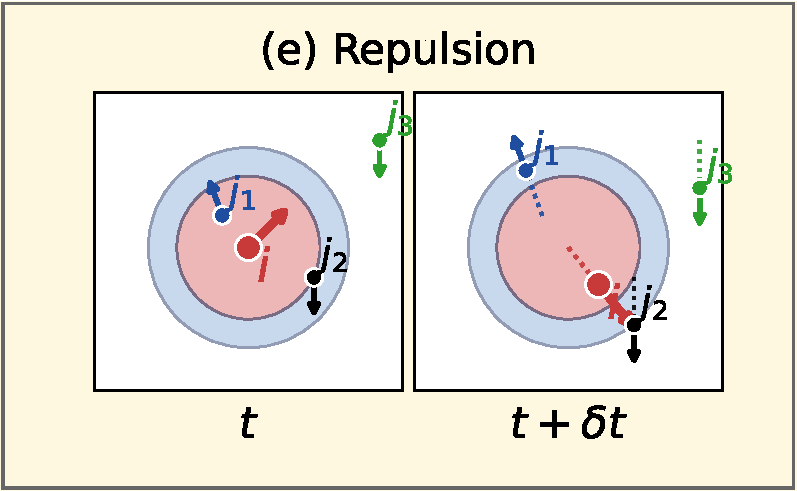
\includegraphics[width=0.32\linewidth]{fig_setup_repulsion.pdf}\hspace{2pt}%
    
\includegraphics[width=0.32\linewidth]{fig_setup_alignment.pdf}
    \caption{Vicsek--Couzin setup and update rules. (a) Two-zone
    geometry around a focal particle: repulsion disc ($d < R_r$),
    alignment annulus ($R_r \leq d < R_a$), full $360^\circ$ vision,
    priority repulsion $\to$ alignment $\to$ inertia. (b) Symmetric
    $\alpha$-stable noise pdfs; smaller $\alpha$ narrows the bulk
    and heavies the tails. (c) The shared sigmoid: $n_i$ sets both
    $v_i$ (purple) and $\alpha_i$ (green), so a crowded particle is
    slow and Gaussian, an isolated one fast and Cauchy. (d)--(f)
    Worked inertia, repulsion and alignment steps of
    Eq.~\eqref{eq:theta_star}, each at $t$ and $t + \delta t$.}
    \label{fig:schematic}
\end{figure}

\subsection{Reference and ablation modes}

The two-feedback model (\emph{double-adaptive}) runs against
three controls on the same code path. Setting $v_{\min} =
v_{\max}$ and $\alpha_{\min} = \alpha_{\max} = 2$ recovers the
original Vicsek dynamics (\emph{Vicsek reference}); setting
instead $\alpha_{\min} = \alpha_{\max} = 1$ gives the
heavy-tailed \emph{Cauchy reference}, the backdrop on top of
which the feedbacks switch on. The \emph{noise-shape only} mode
activates the noise-shape channel with $v_i$ frozen at
$v_{\max}$; the \emph{motility only} mode activates the motility
channel with $\alpha_i$ frozen at the Cauchy value.

\subsection{Order parameters and observables}

The polar order parameter is the magnitude of the average
heading,
\begin{equation}
\langle\varphi\rangle = \Big\langle \frac{1}{N}
   \big|\textstyle\sum_i e^{i\theta_i}\big|\Big\rangle,
\end{equation}
the susceptibility its scaled variance $\chi = N\,
\mathrm{Var}(\varphi)$, and the Binder cumulant $U_4 = 1
- \langle\varphi^4\rangle / (3 \langle\varphi^2\rangle^2)$
\citep{Binder1984}; we read $U_4$ with caution, as every mode
(the Cauchy reference included) drives it to the same
$0.28$--$0.31$ dip, so on its own it does not diagnose the
transition here. For spatial phase separation we use
\begin{equation}
s_{\rm sep} \equiv \max_{\rm bins}\frac{n_{\rm bin}}
   {\mathrm{med}(n_{\rm bin})},
\label{eq:s_sep}
\end{equation}
the ratio of the densest grid cell to the median cell on a
$10 \times 10$ partition: a homogeneous fluid sits at
$s_{\rm sep} \simeq 1$, a phase-separated configuration well
above. A grid-free pair-correlation analogue (the
$95$th-percentile / median ratio of the per-particle local
density within radius $R = 1$) ranks the modes the same way and
ships with the code. To tell a traveling band from an isotropic
patch we use the band-soliton index
\begin{equation}
b \equiv \frac{\max_{x_\parallel} \rho(x_\parallel)}
   {\langle\rho\rangle},
\label{eq:b}
\end{equation}
the maximum of the time-averaged density profile along the
instantaneous polar-flow axis $x_\parallel$ divided by the
spatial mean. A metric-Vicsek traveling band gives
$b \gtrsim 1.5$; an isotropic patch gives $b \simeq 1$.

\subsection{Numerical protocol}

The seven sizes $L \in \{15, 22, 30, 45, 64, 90, 128\}$ run at
fixed density $\rho_0 = N/L^2 = 2.22$, three seeds per
$(\mathrm{mode}, L, \eta)$ cell, with $1500$ warm-up and $1000$
measurement steps from $\theta_i \equiv 0$. The noise grid is
$\eta \in \{0.005, 0.010, 0.020, 0.035, 0.050, 0.075, 0.100,
0.150, 0.200, 0.300\}$, and the fixed parameters are $R_r =
0.5$, $R_a = 0.7$, $n_\star = 3$, $s = 2$, $v_{\min} = 0.005$,
$v_{\max} = 0.05$, $\alpha_{\min} = 1$, $\alpha_{\max} = 2$. The
interaction loop is numba-JIT compiled. A small-$\eta$
refinement $\{0.001, 0.002, 0.003, 0.0075\}$ at the first five
sizes (two seeds) confirms that $\chi_{\max}$ does not lurk
outside the original window, bar the noise-shape-only ablation
at $L = 45$, which we report with its updated value.

\section{Results}
\label{sec:results}

We begin with a visual reference. We show motility-only and
double-adaptive configurations at $\rho_0 = 2.22$, single seed,
after $3000$ warm-up steps, for three sizes $L \in \{30, 90,
128\}$ (one row each) and three noise levels spanning the
ordered ($\eta = 0.020$), near-critical ($\eta = 0.10$) and
disordered ($\eta = 0.30$) regimes (Fig.~\ref{fig:snapshot}).
Deep in the ordered phase the flock is almost fully aligned in
both modes; at near-critical $\eta$ it breaks into locally
ordered slow patches in a faster disordered gas; at $\eta =
0.30$ the particles fill the box with no coherent heading. The
near-critical column is the operating point at which the
rectification below is active, and there the double-adaptive
panels hold a tighter, more coherent dense core than their
motility-only neighbours at every size.

\begin{figure*}[htbp]
    \centering
    
\includegraphics[width=\linewidth]{fig_double_snapshot.pdf}
    \caption{Real-space configurations at $\rho_0 = 2.22$, single
    seed, after $3000$ warm-up steps, three sizes
    $L \in \{30, 90, 128\}$ (one row each). Per row the noise runs
    left to right: (a) $\eta = 0.020$ (ordered), (b) $\eta =
    0.10$ (near-critical), (c) $\eta = 0.30$ (disordered); each
    placing motility-only left of its double-adaptive counterpart.
    Arrows are coloured by local speed $v_i$ (shared colorbar), with
    a $5 \times 5$ zoom inset and the polar order
    $\langle\varphi\rangle$ per panel. Across sizes the
    double-adaptive flock keeps a denser, better-aligned core at
    near-critical and high noise, matching motility-only only deep
    in the ordered phase.}
    \label{fig:snapshot}
\end{figure*}

\subsection{Global diagnostics}
\label{sec:results-global}

\subsubsection{Finite-size scaling of the susceptibility}

To see whether the two adaptations leave a thermodynamic trace
we run all four heavy-tailed modes on the seven-size grid of
Sec.~II~E and read the susceptibility peak $\chi_{\max}(L)$. Its
slope $a$ in $\chi_{\max} \sim L^a$ separates the four modes
(Fig.~\ref{fig:pilot}, Table~\ref{tab:slopes}).

\begin{figure}[htbp]
    \centering
    
\includegraphics[width=0.95\linewidth]{fig_double_pilot.pdf}
    \caption{Seven-size scan, $L \in \{15, 22, 30, 45, 64, 90, 128\}$,
    three seeds, four modes: Cauchy reference (blue), noise-shape
    only (green), motility only (red), double-adaptive (purple).
    Versus $\eta$ at the largest $L$: (a) polar order
    $\langle\varphi\rangle$, (b) susceptibility $\chi$, (c)
    $s_{\rm sep}$, (d) Binder cumulant $U_4$, (f) mean speed
    $\langle v_i\rangle$ (solid) and mean stability
    $\langle\alpha_i\rangle$ (dotted); (e) log--log $\chi_{\max}$
    versus $L$ with fitted slopes. Only the two motility-active
    modes grow a size-dependent $\chi_{\max}$, the double-adaptive
    slope the steeper.}
    \label{fig:pilot}
\end{figure}

The slopes split cleanly into two regimes. The three
fixed-noise-shape modes (Vicsek--Gaussian, Cauchy, noise-shape
only) carry slopes indistinguishable from zero ($-0.04$,
$-0.05$, $-0.01$), every $95\%$ interval straddling the origin
($[-0.08, +0.01]$, $[-0.12, +0.01]$ and $[-0.08, +0.03]$): none
grows a size-dependent susceptibility on the seven-point lever,
the Cauchy-reference $\chi_{\max}$ staying flat near unity. The
two motility-active modes do grow one, and strongly:
$a_{\rm motility} = +1.29$ ($[+1.25, +1.46]$) and $a_{\rm full}
= +1.95$ ($[+1.86, +2.17]$), the full mode steeper and the
intervals disjoint. We read these as the growth rate of a
phase-separation susceptibility, not as critical exponents:
$a_{\rm full} \simeq 2$ means $\chi_{\max} \sim N$, set by a
single phase-separated domain and bounded by the $d = 2$
ceiling, and we find neither a data collapse nor the $U_4$
crossing a genuine critical point would require. The synergy
diagnostic
\begin{equation}
\Delta \equiv (a_{\rm full} - a_{\rm Cauchy})
   - (a_{\rm noise} - a_{\rm Cauchy})
   - (a_{\rm motility} - a_{\rm Cauchy})
\label{eq:delta}
\end{equation}
vanishes for two linearly-combining channels above the Cauchy
backdrop. With the Cauchy and noise-shape slopes both
essentially zero, $\Delta_n$ (on the first $n$ sizes) reduces to
$a_{\rm full} - a_{\rm motility}$, and the full seven-size fit
returns $\Delta_7 = +0.63$, $95\%$ seed-bootstrap interval
$[+0.40, +0.83]$, excluding zero. The interval reflects seed
scatter, not the short lever; and since the $\chi_{\max}$ peaks
already flatten over the largest sizes (motility $37.8 \to 47.7
\to 49.8$ at $L = 64, 90, 128$), we read the $\simeq +0.6$
excess as a finite-size super-additive boost: cooperation
between the channels, not a proven asymptotic exponent. The
load-bearing evidence is the microscopic signature below.

\begin{table}[h]
\centering
\caption{Susceptibility peaks $\chi_{\max}(L)$ on the
seven-size grid and log--log FSS slopes $a$ for the
Vicsek--Gaussian reference and the four heavy-tailed modes,
ten seeds per size (homogeneous protocol). The $95\%$ slope CI
is bootstrapped over the ten seeds ($B = 10\,000$
resamples). The three fixed-noise-shape modes stay flat within
$\pm 0.2$ across the full size range; only the two
motility-active modes grow a size-dependent $\chi_{\max}$, the
double-adaptive slope the steeper.}
\label{tab:slopes}
\small
\begin{tabular}{l c c c c c c c c c}
\toprule
Mode & $L=15$ & $L=22$ & $L=30$ & $L=45$ & $L=64$ & $L=90$ & $L=128$ & slope $a$ & $95\%$ CI \\
\midrule
Vicsek (Gaussian)  & $1.13$ & $1.18$ & $1.07$ & $1.06$ & $1.10$ & $1.08$ & $1.02$ & $-0.04$ & $[-0.08,+0.01]$ \\
Cauchy reference   & $1.05$ & $1.09$ & $1.24$ & $1.06$ & $1.09$ & $0.94$ & $1.04$ & $-0.05$ & $[-0.12,+0.01]$ \\
noise-shape adaptive & $1.19$ & $1.07$ & $1.18$ & $1.11$ & $1.07$ & $1.13$ & $1.15$ & $-0.01$ & $[-0.08,+0.03]$ \\
motility adaptive  & $4.60$ & $5.26$ & $10.07$ & $12.18$ & $37.77$ & $47.66$ & $49.81$ & $+1.29$ & $[+1.25,+1.46]$ \\
double-adaptive    & $3.01$ & $2.31$ & $7.05$ & $21.52$ & $45.27$ & $91.40$ & $93.58$ & $+1.95$ & $[+1.86,+2.17]$ \\
\bottomrule
\end{tabular}
\end{table}

\noindent
The cumulative budget is positive at every truncation and
excludes zero from $n = 5$ onward (per-seed paired $t = +5.9$
at nine d.o.f.). With ten seeds the $\chi_{\max}(L)$ series is
monotone for both motility-active modes, the non-monotonic
$L = 90$ node of the earlier three-seed survey a seed-budget
artefact. The pooled estimator stays seed-sensitive at large
$L$ under heavy tails, which is why the microscopic $g(r)$,
$C(\tau)$, GNF and $P(s)$ diagnostics below carry the
load-bearing evidence.

The reading is mechanistic. Inside a dense patch the alignment
sum over many annulus neighbours is dominated by typical kicks,
so the Cauchy bursts of the heavy-tail-only modes wash out
before they can drive any $\chi_{\max}$ growth. The motility
channel sidesteps that averaging (the dense phase it carves
out has a susceptibility set by density--density fluctuations),
and the noise-shape rectification adds on top because
$\alpha_i \to 2$ damps the residual heading fluctuations in the
same patch, giving the $\Delta a \simeq +0.6$ excess. The $U_4$
panel of Fig.~\ref{fig:pilot}d carries a caveat: all four modes,
the Cauchy reference included, reach the same $U_4 \to
0.28$--$0.31$ dip at $L = 64$. Cauchy fluctuations of the global
order in the dilute phase push $U_4$ down on their own, with no
two-phase coexistence, so the dip is not a reliable first-order
signature here. We turn to $s_{\rm sep}$.

\subsubsection{Density separation and real-space contrast}

The next question is whether the dense regions are spatially
separated. On the same protocol, at the $\chi$-peak $\eta$ and
the three largest sizes (Fig.~\ref{fig:pilot}c), the two
Cauchy-only modes are essentially homogeneous ($s_{\rm sep}
\simeq 1.2$, the binning floor), their $s_{\rm sep}$ in fact
falling slowly with $L$. Only the two motility-active modes
phase separate, both plateauing near $s_{\rm sep} \simeq 1.7$,
the double-adaptive model above the motility-only ablation by
$+0.24$ at $L = 64$ and closing to $+0.01$ by $L = 128$ as they
converge on the plateau. So $s_{\rm sep}$ reads the same split
as the susceptibility slope, with a noise-shape surplus largest
at intermediate sizes before the plateau closes it.

The snapshots (Fig.~\ref{fig:snapshot}, top row, $L = 30$) make
the contrast concrete. At $\eta = 0.020$ the two modes are
almost indistinguishable, $\langle\varphi\rangle = 0.74$
(motility-only) and $0.79$ (full); at near-critical
$\eta = 0.10$ the double-adaptive model already holds more order
($0.52$ against $0.66$); and at $\eta = 0.30$ the motility
ablation collapses to $\langle\varphi\rangle = 0.06$ while the
double-adaptive model still holds $0.39$, its dense slow patches
staying coherently aligned where the motility-only patches
scramble. Inside the
dense phase $\langle\alpha_i\rangle$ reaches $1.5$--$1.6$ for
the full mode and damps the L\'evy bursts that would otherwise
reshuffle the slow particles, whereas the motility-only ablation
takes the full Cauchy kick there at every step: the picture
the shared sigmoid predicts, rectification in the dense regions
and nowhere else.

\subsection{Parametric analyses and distributions}
\label{sec:results-parametric}

\subsubsection{\texorpdfstring{Behavioural plane in $(n_\star, s)$}{Behavioural plane}}

The single working point used so far ($n_\star = 3$, $s = 2$)
sets the strength of both feedbacks. To check that the contrast
extends across the plane we sweep $n_\star$ and $s$ on a $13
\times 13$ grid, three seeds, with a five-point $\eta$ sub-grid
resolving the peaks, at three sizes $L \in \{30, 90, 128\}$
(Fig.~\ref{fig:plane}).

\begin{figure}[htbp]
    \centering
    
\includegraphics[width=\linewidth]{fig_double_plane.pdf}
    \caption{Behavioural $(n_\star, s)$ plane of the
    double-adaptive model, one column per size
    $L \in \{30, 90, 128\}$; top row $\chi_{\max}$, bottom row
    $s_{\rm sep}$; $13 \times 13$ grid, five-point $\eta$ sub-grid,
    three seeds, panels (a)--(f). Cohesion (high $s_{\rm sep}$) and
    the susceptibility maximum peak on different cells, and both
    features persist from $L = 30$ to $L = 128$.}
    \label{fig:plane}
\end{figure}

At $L = 30$ the density-separation map (panel (d)) falls back to
$s_{\rm sep} \simeq 1.5$ in the upper rectangle $n_\star \ge 5$:
the threshold sits past the typical occupancy $\bar n_i \simeq
\rho_0\pi(R_a^2 - R_r^2) \simeq 1.7$ and neither feedback
engages. In the low-threshold band $n_\star \lesssim 3.5$ with
$s \gtrsim 5$ the index climbs to $s_{\rm sep} \approx 2.0$,
peaking near $(n_\star, s) \approx (3.3, 8.5)$, so the cohesion
gain covers the whole MIPS-active corner rather than a
knife-edge cell. The susceptibility map (a) does not
co-localise: its brightest cell sits on the $n_\star = 1$ row,
with $\chi_{\max} = 46$, where $s_{\rm sep}$ has already dropped
to $1.48$. The two optimise on different cells: $\chi_{\max}$
peaks where the threshold sits below typical occupancy and the
rectification fires almost everywhere, washing out the
dense--dilute asymmetry, while $s_{\rm sep}$ peaks where the
threshold bridges typical occupancy and the rectification stays
selective for the dense phase.

Both features survive to $L = 90$ and $L = 128$ (panels (b),
(c) for $\chi_{\max}$; (e), (f) for $s_{\rm sep}$). The
susceptibility ridge stays pinned to the $n_\star = 1$ row and
its peak climbs several-fold above the $L = 30$ value of $46$
(to $\chi_{\max} \simeq 100$--$140$), as expected for a growing
phase-separation susceptibility, while the density-separation
maximum stays in the low-threshold band $n_\star \lesssim 4$,
peaking near $s_{\rm sep} \simeq 1.8$--$1.9$ with the
$n_\star \ge 5$ rectangle still suppressed near $s_{\rm sep}
\simeq 1.2$. The cohesion
gain and its decoupling from the susceptibility peak are
therefore not finite-size artefacts of the small survey boxes.

\subsubsection{\texorpdfstring{Fine-$L$ scan of the transient advantage}{Fine-L scan of the transient advantage}}

To track the $s_{\rm sep}$ gap between the seven FSS nodes we
add five intermediate sizes $L \in \{38, 50, 60, 75, 105\}$ at
five seeds each, with a four-point $\eta$ sub-grid
(Fig.~\ref{fig:Lfine_gap}).

\begin{figure}[htbp]
    \centering
    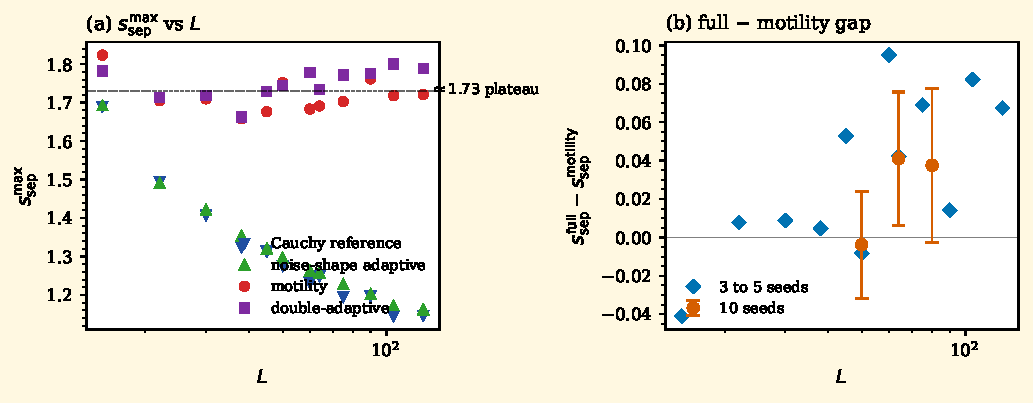
\includegraphics[width=0.92\linewidth]{fig_double_Lfine_gap.pdf}
    \caption{Twelve-size $s_{\rm sep}$ scan: seven-size FSS (three
    seeds) plus five intermediate sizes $L \in \{38, 50, 60, 75,
    105\}$ (five seeds). (a) $s_{\rm sep}^{\max}$ vs $L$ for
    motility-only and double-adaptive; (b) their gap. The surplus is
    significant in an intermediate-$L$ window (sharpest near
    $L = 64$), not monotone in size.}
    \label{fig:Lfine_gap}
\end{figure}

The gap is small at the two smaller fine-grid sizes ($\le
|0.01|$ at $L = 38, 50$) and turns positive in $[+0.07, +0.10]$
across $L = 60$ to $105$, the closure at small $L$ following the
mode-dependent location of the $s_{\rm sep}$ peak in $\eta$. A
ten-seed paired gap at the full-mode $\chi$-peak $\eta$
(Table~\ref{tab:gap_se}) holds the same: $+0.165 \pm 0.031$ at
$L = 64$, but within noise of zero at $L = 50, 80$, so only
$L = 64$ is robustly positive.

\begin{table}[h]
\centering
\caption{Paired $s_{\rm sep}$ gap between double-adaptive
and motility-only at the full-mode $\chi$-peak $\eta$, ten
seeds per cell.}
\label{tab:gap_se}
\small
\begin{tabular}{l c c c}
\toprule
$L$ & gap (full $-$ motility) & SE & z \\
\midrule
$50$ & $+0.020$ & $0.032$ & $+0.64$ \\
$64$ & $+0.165$ & $0.031$ & $+5.28$ \\
$80$ & $+0.024$ & $0.031$ & $+0.77$ \\
\bottomrule
\end{tabular}
\end{table}

The $s_{\rm sep}$ advantage is therefore real and significant at
$L \simeq 64$ but small and seed-budget-limited at neighbouring
sizes. The susceptibility synergy carries the cleanest signature
of the noise-shape contribution, with $s_{\rm sep}$ corroborating
it in the intermediate-$L$ window.

\subsubsection{Transition order, dense-phase geometry, and the Vicsek baseline}
\label{sec:gauss-ref}

Two further checks, detailed in the Supplementary Material, fix
the order of the transition and the geometry of the dense phase.
The order-parameter distribution $P(\langle\varphi\rangle)$
stays unimodal at every size and the quasi-static $\eta$ ramp
opens no hysteresis loop (loop area $\le 0.006$), so the
transition is continuous, or at most very weakly first-order
(Fig.~\ref{fig:transition}). The time-averaged density profile
along the polar-flow axis is flat for all modes (band-soliton
index $b \simeq 1$), so the motility-built dense phase is an
isotropic comoving patch, not a travelling Vicsek band
(Fig.~\ref{fig:profile}).

The four heavy-tailed modes share a Cauchy backdrop and compare
directly; the canonical Vicsek--Gaussian baseline sits outside.
We recover it from Eqs.~\eqref{eq:update}--\eqref{eq:alpha_adapt}
with $v_{\min} = v_{\max} = 0.05$ and $\alpha_{\min} =
\alpha_{\max} = 2$ on the same seven-size, three-seed protocol.
It develops no critical $\chi_{\max}(L)$ scaling at our density:
the peak stays in $1.1$--$1.4$ across the seven sizes, slope
$a_{\rm Vicsek} = +0.01$ ($[-0.09, +0.06]$), the metric-Vicsek
susceptibility damped below the resolution of our lever. The
spatial diagnostic separates more sharply: $s_{\rm sep} = 1.24$
for Vicsek at $L = 64$, nearly identical to Cauchy and
noise-shape ($1.25$), within the homogeneous-fluid range
Cates--Tailleur theory anticipates for a fixed-speed model,
while the full mode lands at $1.72$. The Binder cumulants are
similar across the five modes ($U_4 \in [0.3, 0.5]$).

\subsection{Local diagnostics}
\label{sec:results-local}

\subsubsection{Cluster-size distribution}
\label{sec:clusters}

The cluster-size distribution complements $s_{\rm sep}$: a
homogeneous fluid carries small fluctuations, a spinodal regime
a power-law tail with 2D exponent near $-2$, a binodal regime
one giant cluster coexisting with small ones. We coarse-grain on
a $10 \times 10$ grid, threshold each cell at $1.5$ times the
median occupancy, and run periodic-aware connected-component
labelling on the binary mask; a grid-free DBSCAN check
($\varepsilon = R_a$, four-point core) on the top-density
quartile ranks the modes the same way and ships with the code.
Ten seeds at $L = 30$ separate the four modes
(Figs.~\ref{fig:cluster_summary}, \ref{fig:cluster_map}).


\begin{figure*}[htbp]
    \centering
    
\includegraphics[width=0.95\linewidth]{fig_double_cluster_summary.pdf}
    \caption{Dense-phase structure across the four modes at
    $L = 30$, ten seeds. (a)--(c) seed-averaged cluster count, max
    size and mean size ($\pm 1$ SE): double-adaptive concentrates
    the dense mass into a few large droplets
    ($\langle s_{\max}\rangle = 177$ vs $55$). (d) number
    fluctuations $\mathrm{Var}(N_{\rm box})$ vs
    $\langle N_{\rm box}\rangle$ with fitted $\zeta$ (dashed Poisson
    reference). (e) cluster-size distribution $P(s)$, hue keying the
    mode and line style the noise $\eta \in \{0.02, 0.05, 0.10,
    0.20\}$. Only the motility-active modes phase separate, and the
    rectification redistributes the dense mass into fewer, larger
    droplets.}
    \label{fig:cluster_summary}
\end{figure*}

\begin{figure}[htbp]
    \centering
    
\includegraphics[width=0.95\linewidth]{fig_double_cluster_map.pdf}
    \caption{Real-space cluster identification at near-critical
    $\eta$, single seed, motility-only (top) and double-adaptive
    (bottom) across $L \in \{30, 90, 128\}$ (panels (a)--(f)).
    Dense-bin particles ($> 1.5\times$ median occupancy on a
    $10 \times 10$ grid) are arrows coloured by connected-component
    cluster; dilute-bin particles grey; dense bins ochre-shaded;
    zoom inset per panel. Motility-only fragments the dense phase
    into many clusters; the double-adaptive model concentrates it
    into one or two large droplets at every size.}
        \label{fig:cluster_map}
\end{figure}

The Cauchy and noise-shape modes give only marginal density
fluctuations (a few clusters per seed, max size near the
threshold floor). Both motility-active modes fragment the box
into $\sim 160$--$190$ dense clusters, but the full mode pushes
the largest one far higher (max size $176.6 \pm 42.3$ against
$55.0 \pm 7.5$ for motility-only). Taking the seed as the unit
of replication, and because the dense-phase estimators are
heavy-tailed, we report each full-minus-motility gap with its
$95\%$ seed-bootstrap CI ($B = 10\,000$) and a Wilcoxon
signed-rank test rather than a Gaussian $z$. The two modes
differ on cluster count by $-25.9$ ($[-62.9, +19.5]$, $p =
0.19$; not significant) and on max size by $+121.6$ ($[+40.5,
+206.6]$, $p = 0.02$): the rectification fuses dense patches
into a few large clusters at conserved total dense area
(Fig.~\ref{fig:cluster_map}). Max size is the meaningful
diagnostic; the count carries no clean signal.

The dense-phase distribution $P(s)$ sharpens the same reading
(same $1.5\times$-median dense-bin definition; ten seeds, $L =
30$; $\eta \in \{0.02, 0.05, 0.10, 0.20\}$,
Fig.~\ref{fig:cluster_summary}e). The two fixed-speed references
never grow a dense-phase tail (their giant-cluster fraction
stays at the binning floor, $\langle s_{\max}/N\rangle \simeq
0.001$--$0.002$, the Vicsek band instability at $\rho_0 = 2.22$
too weak to nucleate a dense phase with the motility channel
off), while both motility-active modes carry one. At their
near-critical operating points the double-adaptive tail is the
steeper ($\tau = 2.01$ against $1.74$) with a $2.6$-fold larger
giant-cluster fraction ($0.018$ versus $0.007$), the binodal
signature of mass concentrated into a few large droplets, which
makes the ``fewer, larger droplets'' reading of the cluster map
quantitative.

\subsubsection{Giant number fluctuations}
\label{sec:gnf}

A phase-separated active fluid leaves a second, independent
trace in its density fluctuations. We count the particle number
$N_{\rm box}$ in nested square sub-boxes and read its variance
against the mean, $\mathrm{Var}(N_{\rm box}) \sim \langle
N_{\rm box}\rangle^{2\zeta}$, at $L = 30$, near-critical $\eta$,
ten seeds (Fig.~\ref{fig:cluster_summary}d). A homogeneous fluid
sits at the Poisson value $\zeta = 1/2$; a polar flock reaches
the Toner--Tu value $\zeta \simeq 0.8$. The two fixed-noise-shape
references stay Poissonian ($\zeta = 0.57$ Cauchy, $0.58$
noise-shape), while the two motility-active modes fluctuate
anomalously, $\zeta = 0.79$ (motility-only) and $0.82$
(double-adaptive), both straddling the polar-flock prediction:
the same split read straight off the density fluctuations.

\subsubsection{\texorpdfstring{Heading correlation $g(r)$ in dense and dilute regions}{Heading correlation in dense and dilute regions}}
\label{sec:gr}

If the rectification really acts in the dense phase, its
fingerprint should show up independently of the cluster
geometry. We measure the density-stratified heading
correlation
\begin{equation}
g(r) = \langle \cos[\theta_i(t) - \theta_j(t)] \rangle_{
   |\mathbf x_i - \mathbf x_j| \in [r, r+\Delta r]}
\label{eq:gr}
\end{equation}
for the four heavy-tailed modes at near-critical $\eta$,
$L = 30$, ten seeds with six snapshots per seed. The
reference particle $i$ is restricted to a density quartile of
the local-density field $\rho_i = \#\{j : |\mathbf x_j -
\mathbf x_i| < 1\}$; partner $j$ ranges over the whole box
(Fig.~\ref{fig:gr}).

\begin{figure}[htbp]
    \centering
    
\includegraphics[width=0.95\linewidth]{fig_double_gr.pdf}
    \caption{Density-stratified heading correlation $g(r)$ at
    near-critical $\eta$, $L = 30$, ten seeds. (a) dense and (b)
    dilute quartile for the four modes, with seed-level error bands;
    (c) dense-quartile gap $\Delta g(r)$ between double-adaptive and
    motility-only over $r \in [0.5, 6]$ at $L \in \{30, 64, 90,
    128\}$. The dense correlation is the sharpest fingerprint
    (positive for the motility-active modes, negative for the
    references), and the gap survives all four sizes.}
    \label{fig:gr}
\end{figure}

The dense-phase correlation splits the modes into two groups.
The Cauchy and noise-shape modes reach $g(r \!\simeq\! 0.6) =
-0.169 \pm 0.003$ and $-0.173 \pm 0.004$ in the dense quartile,
both negative: heavy-tailed bursts actively anti-align
particles inside the dense patches. Motility-only reaches $0.542
\pm 0.007$, the full mode $0.695 \pm 0.008$, a paired $\Delta g
= +0.153$ ($95\%$ seed-bootstrap CI $[+0.133, +0.175]$, Wilcoxon
$p = 0.002$). The dilute-phase correlations barely respond to
the noise-shape adaptation, so the asymmetry is the direct
microscopic expression of the rectification, acting where the
shared sigmoid sends it and nowhere else.

The signature survives the FSS range. A ten-seed persistence
test holds the dense-quartile gap in $\Delta g(r \!\simeq\! 0.6)
\in [+0.11, +0.15]$ across $L = 64$ to $128$ (each $95\%$
seed-bootstrap CI excluding zero, Wilcoxon $p = 0.002$),
narrowing mildly from $+0.15$ at $L \le 64$ to $+0.11$ at
$L = 128$. Over the full $r \in [0.5, 6]$ profile
(Fig.~\ref{fig:gr}c) it does not decay with $r$: the outer-range
mean ($r > 3$, $+0.14$ to $+0.18$ across sizes) sits if anything
above the inner-range mean ($r \in (0.5, 1.5)$, $+0.11$ to
$+0.15$), larger beyond the alignment cutoff $R_a = 0.7$ than
inside it. The rectification imposes a coherence on the dense
phase that outlasts the metric interaction range.

\subsubsection{\texorpdfstring{Single-particle dynamics: $C(\tau)$, turning angles and diffusion}{Single-particle dynamics: C(tau), turning angles and diffusion}}
\label{sec:autocorr}

The dense $g(r)$ measures the static sharpness of local
alignment but says nothing about how a heading evolves. Three
single-particle diagnostics, all on the same near-critical runs
at $L = 30$, $\rho_0 = 2.22$, close that gap and pin the
mechanism behind the macroscopic gains (Fig.~\ref{fig:dynamics}).
We start with persistence. The appendix (Sec.~\ref{sec:hydro})
predicts a rotational decorrelation
rate $\Gamma(\rho, \eta) \simeq \eta^{\alpha(\rho)}$: $\eta^2$
inside the dense phase ($\alpha \to 2$), $\eta$ in the dilute
one ($\alpha \to 1$), a factor $\eta^{-1} \simeq 10$ at our
working point. For each mode at its near-critical $\eta$, ten
seeds, $n_{\rm meas} = 20\,000$ steps, we tag every particle
every $50$ steps by quartile of the local count and compute
$C_{\rm dense}(\tau) = \langle \cos[\theta_i(t+\tau) -
\theta_i(t)] \rangle_{i \in \text{dense}}$ on lags $\tau \in
\{1, 2, 5, 10, 20, 50, 100, 200, 500, 1\,000, 2\,000, 5\,000\}$
(and similarly $C_{\rm dilute}$). The four modes order the same
way at every lag (Fig.~\ref{fig:dynamics}a): Cauchy and
noise-shape drop fastest, motility-only sits above, and the
full model sits above motility-only by a nearly constant
offset. The gap $\Delta C(\tau) = C_{\rm full}(\tau) -
C_{\rm motility}(\tau)$ stays in the band $+0.13$ to $+0.24$
over $\tau \in [1, 5\,000]$ in the dense quartile, its bootstrap
$95\%$ CIs (ten seeds, $B = 10\,000$ resamples) excluding zero
throughout. The within-seed estimator averages over $\sim 4
\times 10^7$ sample pairs per mode, so we quote bootstrap CIs
rather than a between-seed $z$, which saturates beyond a few
sigmas. The dilute gap is a few percent and its CI brackets zero
past $\tau \simeq 100$.

\begin{figure}[htbp]
    \centering
    
\includegraphics[width=\linewidth]{fig_double_dynamics.pdf}
    \caption{Single-particle dynamics at $L = 30$, $\rho_0 = 2.22$,
    near-critical $\eta$. Top row (ten seeds, $20\,000$ steps): (a)
    $C_{\rm dense}(\tau)$ per mode ($\pm 1$ SE bands); (b) the gap
    $\Delta C(\tau) = C_{\rm full} - C_{\rm motility}$ in the dense
    and dilute quartiles, with $z$-scores. Bottom row, per-particle
    increments (six seeds; hue keys the mode, line style the density
    class, solid dense, dashed dilute): (c) turning-angle pdf
    $p(\Delta\theta)$; (d) density-conditioned MSD
    $\langle\Delta r^2\rangle(\tau)$ with fitted
    $\gamma_{\rm dense}/\gamma_{\rm dilute}$. The dense $C(\tau)$
    gap persists far beyond the polar-order correlation time; only
    the double-adaptive increment turns Gaussian-narrow in the dense
    phase ($\alpha \to 2$), and that dense phase is ballistic
    ($\gamma \simeq 2$) while the dilute gas is super-diffusive but
    sub-ballistic. The noise gate switches dense-phase reorientation
    from L\'evy-like to Gaussian, but only once the motility channel
    has built the dense phase.}
    \label{fig:dynamics}
\end{figure}

The dense-phase plateau matches the $\Gamma \simeq
\eta^{\alpha(\rho)}$ form of Sec.~\ref{sec:hydro_fields}: a more
persistent heading once $\alpha$ switches from $1$ to $2$ inside
the motility-built dense phase. Measured at a single $\eta$ per
mode and flat across lags, the gap probes the dense-phase
$\alpha \to 2$ conversion, not the $\eta$-exponent of $\Gamma$
itself, which an $\eta$-resolved run would be needed to test.
$C(\tau)$ thus extends the static dense $g(r)$ of
Fig.~\ref{fig:gr}c to the single-particle dynamic, at lags well
beyond the polar-order correlation time.

The per-step turning-angle distribution then exposes what the
persistence plateau rests on: the noise gate is a switch in the
reorientation statistics. Stratifying the same runs by
density quartile (six seeds, $8\,000$ steps;
Fig.~\ref{fig:dynamics}c, solid dense, dashed dilute), in the
dilute gas both motility-active models turn with a heavy,
Cauchy-like tail (weight beyond $|\Delta\theta| > \pi/2$ of
$0.34$ double-adaptive, $0.41$ motility-only). In the dense
phase they part company: the double-adaptive increment collapses
onto a Gaussian-like core (tail weight $0.14$, circular variance
$0.34$), whereas motility-only stays heavy (tail weight $0.22$,
circular variance $0.50$) with $\alpha$ pinned at $1$. The gate
cuts the dense tail weight by $2.4$ for the double-adaptive
model against $1.9$ for motility-only: the $C(\tau)$ plateau,
read at the level of increments, is a switch from heavy-tailed
to Gaussian turning inside the dense phase. The two fixed-speed
references keep a heavy dense-quartile tail, so the Gaussian
conversion needs the motility channel to build the dense phase
first.

The stratified mean squared displacement
$\langle\Delta r^2\rangle(\tau)$, conditioned on the density
class at the time origin and unwrapped across the periodic box,
turns this into transport (Fig.~\ref{fig:dynamics}d). The dense
phase is ballistic (a coherent, comoving ordered droplet),
with exponent $\gamma_{\rm dense} = 2.01 \pm 0.01$ for the
double-adaptive model and $1.93$ for motility-only, while the
dilute gas is super-diffusive but sub-ballistic,
$\gamma_{\rm dilute} = 1.59$ and $1.45$, the fast free particles
losing direction to their heavy-tailed turning. The two
fixed-speed references stay near-diffusive ($\gamma \simeq
1.0$--$1.1$ in both quartiles): building no dense phase, their
fast but heavy-tailed motion simply randomises. The double
feedback raises the exponent in both phases and lifts the
dense-phase displacement at $\tau = 2\,000$ steps by $66\%$
($235.7$ against $142.2$ in box units): the Gaussian gate makes
the dense droplets advance as cleaner ballistic units. The
noise channel sets the turning statistics (Gaussian and
directed inside the dense flock, heavy-tailed in the dilute
gas), the speed channel sets the magnitude, and together they keep
the double-adaptive droplets denser, more cohesive and more
persistent than the motility-only ablation.

\subsubsection{Decoupled sigmoids: a four-way anatomy of the rectification}
\label{sec:decoupled}

The shared sigmoid cannot say which ingredient does the work.
We split it into two independent profiles and run four tests:
the threshold plane (Sec.~\ref{sec:decoupled-map}), the density
dependence (Sec.~\ref{sec:decoupled-sigma}), the alignment
kernel (Sec.~\ref{sec:decoupled-topo}) and the patch
persistence (Sec.~\ref{sec:decoupled-lifetime}).

\label{sec:decoupled-map}
We replace the shared sigmoid by two independent ones with
parameters $(n_\star^v, s^v)$ and $(n_\star^\alpha,
s^\alpha)$; setting both thresholds to $3$ and both slopes to
$2$ recovers the shared model. Sweeping the quadrant
$(n_\star^v, n_\star^\alpha) \in \{1, 2, 3, 5, 8\}^2$ at fixed
$s^v = s^\alpha = 2$, ten seeds per cell at $L = 30$, $\eta =
0.15$, we record the seed-paired gap $\Delta g(r \!\simeq\! 0.6)
= g_{\rm full}^{\rm decoupled} - g_{\rm motility}$
(Fig.~\ref{fig:decoupled_2d}).

\begin{figure*}[htbp]
    \centering
    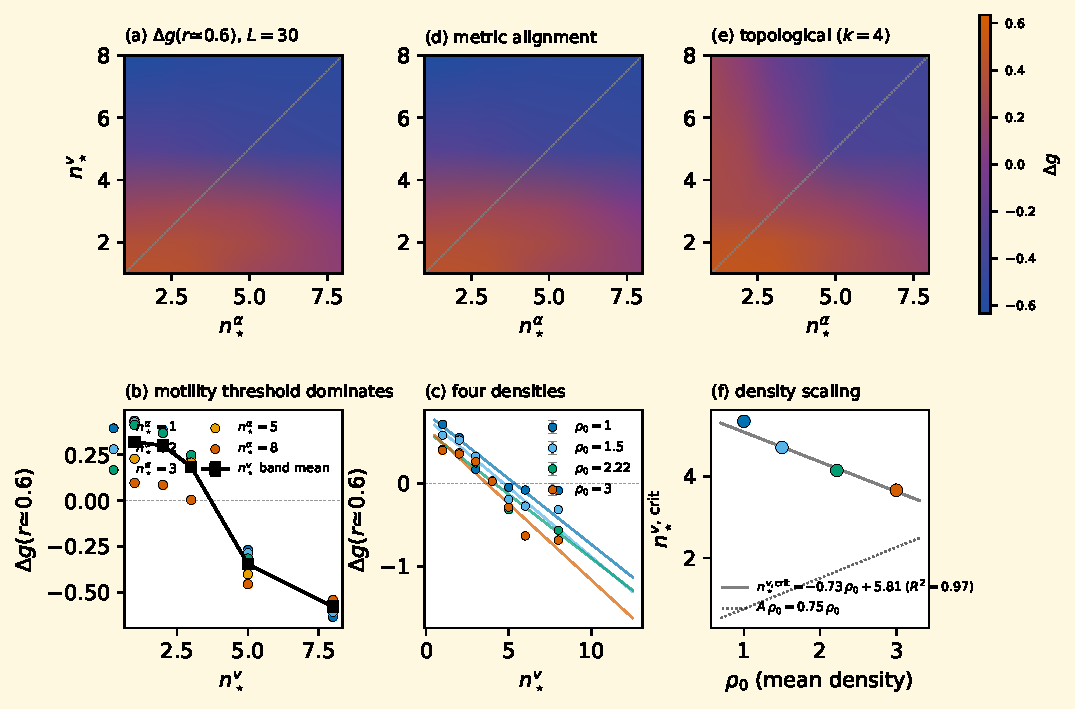
\includegraphics[width=0.98\linewidth]{fig_double_decoupled_2d.pdf}
    \caption{Decoupled-sigmoid dissection of the gap
    $\Delta g(r\!\simeq\!0.6) = g_{\rm full}^{\rm decoupled} -
    g_{\rm motility}$ at $L = 30$, ten seeds per cell. (a) Heatmap
    on the $(n_\star^\alpha, n_\star^v)$ plane (dashed
    $n_\star^v = n_\star^\alpha$). (b) $\Delta g$ vs $n_\star^v$
    keyed by $n_\star^\alpha$, with band means ($\pm 95\%$ CI)
    crossing zero at $n_\star^v \simeq 4$ ($R^2 = 0.88$ on
    $n_\star^v$ vs $0.04$ on $n_\star^\alpha$). (c) Density-scaling
    test at $\rho_0 \in \{1.0, 1.5, 2.22, 3.0\}$ ($n_\star^\alpha =
    3$). (d) Metric and (e) topological ($k = 4$) heatmaps at
    $\rho_0 = 2.22$, matched scale. (f) Critical threshold
    $n^{v,\,{\rm crit}}_\star(\rho_0) = -0.73\,\rho_0 + 5.81$
    ($R^2 = 0.97$; dotted, mean-density prediction $A\rho_0$). The
    sign is set by $n_\star^v$ alone and only for the metric kernel,
    marking the rectification as a metric, motility-driven effect.}
    \label{fig:decoupled_2d}
\end{figure*}

The map splits the quadrant into two horizontal bands,
separated not by the diagonal but by a critical motility
threshold $n_\star^v \simeq 4$, just above the typical
alignment-zone occupancy $\rho_0\pi(R_a^2 - R_r^2) \simeq
1.7$. Averaging each $n_\star^v$ band over $n_\star^\alpha$, the
mean gap steps monotonically with the motility threshold, from
$+0.32$ ($95\%$ seed-bootstrap CI $[+0.31, +0.33]$) at
$n_\star^v = 1$ down to $-0.58$ ($[-0.59, -0.57]$) at $8$, the
adjacent bands non-overlapping and the sign flipping at
$n_\star^v \simeq 4$.
The matching $n_\star^\alpha$ bands stay near zero ($+0.03$
for $n_\star^\alpha \le 3$, down to $-0.16$ at
$n_\star^\alpha = 8$), so the noise-shape threshold is
passive. The shared-sigmoid diagonal ($n_\star^v =
n_\star^\alpha$) crosses straight from the positive bands at
$n_\star^v \le 3$ to the negative bands at $n_\star^v \ge 5$,
so the sign is set by $n_\star^v$ alone, not by the timing
offset; a linear fit corroborates it ($\Delta g \simeq
-0.144\, n_\star^v + 0.52$, $R^2 = 0.88$, against $R^2 = 0.04$
on $n_\star^\alpha$ and $0.28$ on the timing offset).

The mechanism is simple. At $n_\star^v = 3$, just above typical
occupancy, dense-patch particles fire the motility channel while
the rest saturate at $v_{\max}$. Push $n_\star^v$ to $5$ or $8$
and the motility channel almost never fires: the decoupled model
collapses onto the noise-shape-only ablation, which has
$g(r\!\simeq\!0.6) = -0.17$ at $L = 30$ (Sec.~\ref{sec:gr}), and
its gap with motility-only is large and negative, the lower
band. Drop $n_\star^v$ below $3$ and the motility channel
engages aggressively; dense patches grow and the noise-shape
rectification adds coherence on top whether it triggers early or
late, giving the upper band. The slowdown is again the
precondition: heavy-tailed reorientations sharpen cohesion the
motility channel has already laid down, never cohesion of their
own.

\label{sec:decoupled-sigma}
How does the critical motility threshold
$n_\star^{v,{\rm crit}}$ move with the global density $\rho_0$?
The mean-density reading takes the relevant count to be $A\rho_0
= \pi(R_a^2 - R_r^2)\,\rho_0$ and predicts $n_\star^{v,{\rm
crit}} \propto \rho_0$ with slope $A \simeq +0.75$. We test that
by sweeping $n_\star^v \in \{1, 2, 3, 4, 5, 6, 8\}$ at three
extra densities $\rho_0 \in \{1.0, 1.5, 3.0\}$ (plus $\rho_0 =
2.22$), $n_\star^\alpha = 3$ fixed, ten seeds, reading off the
zero crossing of $\Delta g(n_\star^v) \simeq a(\rho_0)\,
n_\star^v + b(\rho_0)$. Per-density fits all reach $R^2 \ge
0.86$ (Fig.~\ref{fig:decoupled_2d}b) and
\begin{equation}
n_\star^{v,{\rm crit}}(\rho_0)
   = -0.73\,\rho_0 + 5.81,
\qquad R^2 = 0.97.
\label{eq:nv_crit_sigma}
\end{equation}
The mean-density prediction is wrong in sign:
$n_\star^{v,{\rm crit}}$ falls with $\rho_0$, the slope
$-0.73$ the mirror image of $+0.75$.

The reversed sign most likely traces to the dense-to-dilute
density contrast, a phenomenological reading we leave for a
first-principles account (App.~\ref{sec:hydro}). At low $\rho_0$
the dilute phase is nearly empty, the dense phase carries a
large relative contrast, and its local count clears even a
demanding $n_\star^v \simeq 5$; at high $\rho_0$ the dilute
phase is itself crowded, the contrast weakens, and $n_\star^v$
must drop to stay selective. Extrapolating
Eq.~\eqref{eq:nv_crit_sigma} to $\rho_0 \simeq 8$ gives
$n_\star^{v,{\rm crit}} \to 0$: once the two phases are
indistinguishable, no threshold buys a coherence gain. The
naive alternative fails a falsification check: if
$n_\star^{v,{\rm crit}}$ tracked the dense-phase neighbour count
$\langle n_i\rangle_{\rm dense}$ the two would be equal, but
$\langle n_i\rangle_{\rm dense}$ \emph{increases} with $\rho_0$
(from $2.6$ at $\rho_0 = 1.0$ to $5.3$ at $\rho_0 = 3.0$),
opposite to $n_\star^{v,{\rm crit}}$.


\label{sec:decoupled-topo}
Metric alignment conflates two roles: the sigmoid input $n_i$
and the partner set are the same object. We pull them apart with
the topological variant of \citet{Ginelli2010}, where each
particle aligns with its $k$ nearest non-repulsion neighbours
while the sigmoid input stays the metric annulus count.
Re-running the $25$-cell map at $L = 30$, $\rho_0 = 2.22$ with
$k = 4$ (Fig.~\ref{fig:decoupled_2d}c), the two-band structure
softens. The linear fit on $n_\star^v$ alone drops from $R^2 =
0.88$ to $0.68$ while the $n_\star^\alpha$ fit climbs from
$0.04$ to $0.43$, the bivariate fit now splitting its weight
nearly evenly between the two thresholds. The sign-flip region
retreats too: cells that were strongly negative under metric
alignment turn positive, only the high-high corner staying
negative.

So motility-threshold dominance is a property of the metric
kernel, not of the two-feedback dynamics. Under metric alignment
$n_{\rm ali}$ both feeds the sigmoid and selects the alignment
partners, so pushing the threshold above typical occupancy
switches off the slowdown and the neighbour-driven alignment at
once. Topological alignment breaks that tie: the $k = 4$ nearest
neighbours hand each particle a baseline alignment the
rectification can sharpen even when the motility channel is
nearly silent. The model thus speaks sharpest to short-metric
perceivers (swarming bacteria, insects in dense plumes), less so
to topological ones (starlings, schooling fish).

\label{sec:decoupled-lifetime}
The full-mode droplets are larger; are they longer-lived? We
track the centroids of the connected dense components over $200$
snapshots spaced $50$ steps, matching across snapshots by
periodic-centroid distance (cutoff $4.0$) and particle-count
ratio (cutoff $2.0$), ten seeds. The mean patch lifetime is
$1.60$ snapshots in motility-only against $1.57$ in the full
mode, a difference of $-0.034$ ($95\%$ bootstrap CI $[-0.10,
+0.03]$, Mann-Whitney $p = 0.08$; not significant). The
geometric consolidation buys no temporal persistence: the
rectification reshapes which cells the dense particles occupy at
each instant while leaving cell turnover to the motility
dynamics. It acts on geometry, not persistence.

Together the four tests pin the rectification down. It is a
spatial consolidation that needs an aggressive motility
threshold and a metric kernel to engage; under those conditions
it works regardless of the noise-shape threshold, never extends
patch lifetimes, and switches off once the global density washes
out the dense-to-dilute contrast. It piggybacks on the MIPS
instability rather than driving the phase separation itself.

\section{Discussion}
\label{sec:disc}

\subsection{Mechanism and biological reading}
\label{sec:disc-mechanism}

What ties the two channels together is the shared sigmoid in
$n_i$: speed and stability index move in lockstep. Inside a
dense patch the sigmoid pushes $\alpha_i \to 2$, replacing the
Cauchy bursts that would otherwise scramble a slow particle by
Gaussian-like kicks. A rectified kick no longer randomises the
local alignment, so the noise-shape channel acts as a
fluctuation rectifier \emph{inside} the slow region the motility
channel carves out. The two adaptations cooperate where it
matters and never fight locally. The finite-size susceptibility
carries a positive but partly saturating super-additive excess;
the robust faces are microscopic: the dense $g(r)$, its
dynamic counterpart $C(\tau)$, and the cluster geometry, all
significant at $L = 30$ and all flat in the dilute quartile. The
decoupled-sigmoid tests of Sec.~\ref{sec:decoupled} sharpen the
picture: the rectification is a spatial consolidation, not a
temporal stabilisation ($p = 0.08$); it needs the metric kernel
($n_\star^v$ dominance weakening from $R^2 = 0.88$ to $0.68$
under topological alignment); the motility threshold controls it
alone; and it switches off once the dense-to-dilute contrast
washes out ($n_\star^{v,{\rm crit}} \to 0$ as $\rho_0 \to 8$).

The biological reading carries an unambiguous priority. A flock
that slows down aggressively reaps the two-feedback cohesion at
almost any noise-shape threshold, whereas a flock with an inert
motility channel lets the noise-shape adaptation damage
dense-phase coherence. The link to locust marching
\citep{Buhl2006, Bazazi2008} and to swarming fish or starling
flocks at sub-thermodynamic sizes follows from that.

\subsection{Literature, limits and outlook}
\label{sec:disc-literature}

The motility channel inherits directly from
\citet{CatesTailleur2015}: our motility-only ablation reproduces
$\partial \ln v / \partial \ln \rho < -1$ MIPS inside an
aligning Couzin flock, with $s_{\rm sep}$ rising from $\simeq
1.2$ for the fixed-speed references to $\simeq 1.7$. This is in
the spirit of \citet{Bi2016}'s density-driven epithelial
jamming, but we keep the alignment interaction, so the dense
phase is polar rather than amorphous. Within the metric-Vicsek
lineage of \citet{Vicsek1995}, \citet{Gregoire2004} and
\citet{Chate2008} established traveling bands and a weakly
first-order transition; the band-soliton index $b \le 1.06$
(Fig.~\ref{fig:profile}) shows we never reach that regime, and
$P(\langle\varphi\rangle)$ stays unimodal at $L = 30$ with $U_4
\simeq 0.65$ in both motility-only and full modes. The
Toner--Tu programme \citep{TonerTu1995, TonerTu1998,
TonerTu2012} predicts the same continuous polar order but does
not anticipate the dense-quartile gap of Fig.~\ref{fig:gr},
treating the noise as Gaussian with density-independent
variance. The $\Delta a \simeq +0.6$ gap between the full and
motility-only slopes is a quantitative target for a
density-dependent Toner--Tu closure.

The heavy-tail strand is the second axis. \citet{Reynolds2018},
\citet{Harris2012} and \citet{Ariel2015} document L\'evy
reorientations in foragers, T-cells and swarming bacteria. Our
noise-shape ablation tempers the heavy-tail-as-driver picture:
the Cauchy and noise-shape modes carry slopes statistically
indistinguishable from zero, so heavy-tailed reorientations on
their own grow no size-dependent $\chi_{\max}(L)$ at our
density: the alignment averaging in the dense phase washes the
bursts out. The motility channel is necessary, heavy tails alone are
not sufficient, and what the noise-shape adaptation buys is the
cooperative $\Delta_n > 0$ on top of the motility-driven
scaling. Where \citet{Couzin2002} treats the zonal parameters as
global constants, we make the stability index a local field on
the same kernel. \citet{Bechinger2016} and \citet{Marchetti2013}
review and embed such feedbacks hydrodynamically, but neither
identifies the dense-phase Gaussian conversion, because neither
couples the noise distribution to the local density. The two
ingredients are documented separately: a density-dependent
speed across active colloids, traffic and jamming
\citep{CatesTailleur2015, Greenshields, Bi2016}, and
environment-dependent reorientation statistics in swimming
bacteria \citep{Korobkova2004, Dieterich2008}. Swimming
bacteria, where crowding both slows the cells and reshapes their
tumble statistics, are the closest concrete instance of the two
responses coexisting, though they need not share a single
sensor. The shared sigmoid is in that sense a parsimony
assumption, not a documented mechanism; its sharpest prediction,
a dense-phase narrowing of the turning-angle distribution
together with a positive heading-correlation gap, is what an
experiment on a crowding-responsive collective could test.

The weakest part of the case is the lever. The seven-size FSS is
short: the excess is positive at every budget and excludes zero
from $n = 5$ onward ($\Delta_7 = +0.63$, $[+0.40, +0.83]$), but
the $\chi_{\max}$ peaks already flatten at the largest sizes, so
we read it as a finite-size boost rather than an asymptotic
exponent. Controlled runs at $L = 180$ or $256$ with an explicit
data collapse would test whether the excess slope holds
asymptotically and whether $P(\langle\varphi\rangle)$ narrows.
Mapping $g(r)$ at intermediate distances $r = 2$ to $5$ would
tell whether the rectification carries a characteristic decay
length, in the spirit of \citet{Eliazar2003}, and the absence of
a traveling band leaves room for a different cohesive structure,
perhaps a slowly-rotating dense droplet, that a real-space
analysis at $L > 30$ should reveal. On the theory side, a
Toner--Tu closure with $v_{\rm eff}(\rho)$ and a fractional
$D_{\rm rot}(\rho) \propto \eta^{\alpha(\rho)}$ recovering both
the linear $\Delta g(n_\star^v)$ and the negative slope
$n_\star^{v,{\rm crit}}(\rho_0) = -0.73\,\rho_0 + 5.81$ would
close the mechanistic argument.

\appendix

\section{A heuristic hydrodynamic sketch and the decoupled-sigmoid asymmetry}
\label{sec:hydro}

The model coarse-grains to fields $\rho(\mathbf x, t)$ and
$\mathbf p(\mathbf x, t) = \rho^{-1}\langle\vec e_i\rangle_x$.
The treatment is heuristic: it makes the rectification
analytically transparent, not derived.

\subsection{Continuum fields and conservation}
\label{sec:hydro_fields}

With the continuum neighbour count $n_i \approx A\,\rho$,
$A \equiv \pi(R_a^2 - R_r^2) \simeq 0.75$,
Eqs.~\eqref{eq:sigmoid}--\eqref{eq:alpha_adapt} become density
fields,
\begin{align}
\sigma(\rho) & = \frac{1}{1 + \exp\!\bigl[-s\,(A\rho - n_\star)\bigr]},
\label{eq:sigma_rho} \\
v(\rho) & = v_{\max} - \Delta v\,\sigma(\rho),
\quad \Delta v \equiv v_{\max} - v_{\min},
\label{eq:v_rho}
\end{align}
and $\alpha(\rho)$ likewise interpolating from $\alpha_{\min}$
to $\alpha_{\max}$. Density conservation and the polarisation
dynamics read
\begin{equation}
\partial_t \rho + \nabla\!\cdot\!\bigl[\rho\,v(\rho)\,
\mathbf p\bigr] = 0,
\label{eq:rho_eq}
\end{equation}
\begin{equation}
\partial_t \mathbf p = -\Gamma(\rho, \eta)\,\mathbf p
   + \nu\,\nabla^2\mathbf p
   - \lambda\,(\mathbf p\!\cdot\!\nabla)\mathbf p
   + \cdots,
\label{eq:p_eq}
\end{equation}
with $\nu, \lambda$ the standard Toner--Tu coefficients
\citep{TonerTu1995, TonerTu2012}. The non-trivial input is that
the decorrelation rate $\Gamma$ depends on $\rho$ through
$\alpha(\rho)$.

\subsection{Effective rotational decorrelation}

A symmetric $\alpha$-stable kick gives $\langle\cos\xi\rangle =
\exp(-\eta^\alpha)$, so for small $\eta$
\begin{equation}
\Gamma(\rho, \eta) = 1 - \langle\cos\xi\rangle
   \;\simeq\; \eta^{\alpha(\rho)}.
\label{eq:gamma_eta}
\end{equation}
This is $\eta$ in the dilute (Cauchy) limit and $\eta^2$ in the
dense (Gaussian) one: the noise-shape feedback turns the
$\eta$-linear Cauchy decorrelation into the much weaker $\eta^2$
Gaussian one inside the dense phase, the analytic counterpart of
the rectification.

\subsection{MIPS instability and its rectification correction}

A homogeneous polar state goes unstable under a longitudinal
density perturbation by the Cates--Tailleur mechanism
\citep{CatesTailleur2015} when
\begin{equation}
\frac{\partial \ln v(\rho)}{\partial \ln \rho}\bigg|_{\rho_0}
   < -1,
\label{eq:CT_criterion}
\end{equation}
which the sigmoidal $v(\rho)$ meets in a window of width $1/s$
centred on $A\rho_0 \simeq n_\star$. Since $v$ and $\alpha$
share the sigmoid, that window coincides with the density at
which the rectification fires, so the nucleating dense phase is
born already rectified.

The sketch has a real limit, which we concede. A sequential
timing argument predicts only the diagonal ordering of the
decoupled map, whereas the data run along horizontal lines of
constant $n_\star^v$ (Fig.~\ref{fig:decoupled_2d}, $R^2 = 0.88$
against $0.28$ for the timing-offset fit). Neither the
horizontal-band structure nor the negative slope
$n_\star^{v,{\rm crit}}(\rho_0) = -0.73\,\rho_0 + 5.81$ follows
from the linear-stability picture; recovering both from
Eqs.~\eqref{eq:rho_eq} and \eqref{eq:p_eq} would need the
dense-phase density tied to the MIPS contrast rather than to the
mean, which we leave to a quantitative theory.

\section*{Code and data availability}
The simulation code, all run drivers, the
figure-generation scripts and the precompiled data are openly
available at
\url{https://github.com/yayayou47/two-feedback-vicsek} under
the \textsc{mit} license, and will be archived on Zenodo with
a permanent DOI on acceptance. All runs used
Python~3.12.3, NumPy~2.4.4, SciPy~1.17.1, Numba~0.65.1
(LLVM~0.47.0) and Matplotlib~3.10.9 on Linux x86\_64. The
interaction loop is JIT-compiled with Numba's parallel
reduction; per-particle random streams are derived from a
single NumPy \texttt{Generator} with a per-run seed, so
each \texttt{(seed, mode, $L$)} tuple is reproducible
bit-for-bit. A movie utility ships alongside the run drivers
and writes MP4 sequences for each mode with frames coloured
by $v_i$ and an inset tracking $\langle\varphi\rangle(t)$
and $s_{\rm sep}(t)$.

\bibliographystyle{iopart-num}
\bibliography{refs}


\end{document}
